\vspace*{1.5pc}

In this section, I detail the results we obtain on the mass of dark matter particles in the context of two projects I explored. The first, presented in Sec.~\ref{sec:pureWDM}, incorporates sterile neutrinos (and thermal relics) as a pure WDM particle. In the second, presented in Sec.~\ref{sec:res_rpsn}, I allowed for lepton asymmetries to boost the production of neutrinos as a pure cool dark matter candidate particle. 


\subsection{Warm Dark Matter}
\label{sec:pureWDM}

Establishing constraints on WDM candidate particle masses using the Ly-$\alpha$ power spectrum was done in many studies previous to my own; \textit{e.g.} \cite{VLH08a, VLH08b, SMT08, VBH08, BLR09, VBH13} amongst others. The lower bounds on WDM mass in each of these works is summarized in Tab.~\ref{tab:studies}. 

\begin{table}
	\begin{center}
	\rotatebox{90}{
		\begin{tabular}{llllll}
			\textbf{Reference} & \textbf{QSO spectra} & \textbf{Data} & \textbf{Simultion} & \textbf{Bounds on $m_{\nu_s}^{\rm{nrp}}$} & \textbf{Tension with}\\[2pt]
			\textbf{study} & \textbf{resolution} & \textbf{set} & \textbf{resolution} & \textbf{from Ly-$\alpha$ forests} & \textbf{X-ray bounds}\\[2pt]
			\hline \\[-10pt]
			\cite{SMT08} & low only & SDSS-I & 12.8 (hydro)& $\geq~12$ keV & $6~\sigma$\\[2pt]
			\cite{BLR09} & low + high & SDSS-I + UVES & 6.7 (N-body) & $\geq~10$ keV& $5~\sigma$\\[2pt]
			\cite{VBH13} & high only & HIRES + MIKE & 25.6 (hydro) & $\geq~19$ keV& $9.5~\sigma$\\[2pt]
			\cite{Baur16} & low only & SDSS-III & 30.72 (hydro) & $\geq~24$ keV& $12~\sigma$\\[2pt]
			\cite{Yeche17} & low + medium & SDSS-III + XQ100 & 30.72 (hydro) & $\geq~25$ keV& $12.5~\sigma$\\[2pt]
			\cite{IrsicWDM} & medium + high & XQ100 + MIKE & 38.4 (hydro) & $\geq~34$ keV& $17~\sigma$\\[2pt]
			\hline \\[-10pt]
		\end{tabular}
	}
	\end{center}
	\caption{Summary of Ly-$\alpha$ constraints on NRP neutrino mass according to the data set used. Quoted lower bounds are the 95\% confidence level. Tension with the upper bound from X-rays is expressed in standard deviations in the right-most column. Simulation resolution refers to the quantity $\frac{N}{L / \rm{Mpc}}$.}
	\label{tab:studies}
\end{table}

%\begin{table}
%\begin{center}
%\begin{tabular}{lccll}
%\textbf{Reference} & \multicolumn{2}{c}{\textbf{$95\%$ C.L. lower bound}} & \textbf{QSO spectra data set} & \textbf{Simulations} \\[2pt]
%. & $m_x/\mathrm{keV}$ & $m_{\nu_s}^{\mathrm{nrp}}/\mathrm{keV}$ & . & ($L/h^{-1}\mathrm{Mpc}$, $N$) \\[2pt]
%\hline \\[-10pt]
%VLH05 \cite{VLH08a} & $0.55$ & $1.8$ & 30 HIRES + 27 UVES + 23 LRIS & (30, 200) hydro\\[2pt]
%VLH06 \cite{VLH08b} & $2.0$ & $9.7$ & 3035 SDSS & (20, 256) hydro\\[2pt]
%BLR09 \cite{BLR09} & $2.1$ & $10.4$ & 57 UVES + 3035 SDSS & (60, 400) N-body\\[2pt]
%SMT06 \cite{SMT08} & $2.4$ & $12.2$ & 3035 SDSS & (20, 256 gas 512 DM) hydro\\[2pt]
%VBH13 \cite{VBH13} & $3.3 $ & $18.5$ & 14 HIRES + 11 MIKE & (20, 512) hydro\\[2pt]
%VBH08 \cite{VBH08} & $4.0$ & $23.7$ & 55 HIRES + 3035 SDSS & (60, 400) + (20, 256) hydro\\[2pt]
%This work & $4.1$ & $24.4$ & 13,821 SDSS-III & (100, 3072) hydro\\[2pt]
%This work & $3.0$ & $16.0$ & 13,821 SDSS-III + Planck & (100, 3072) hydro\\[2pt]
%\hline \\[-10pt]
%\end{tabular}
%\end{center}
%\caption{Summary of past lower bounds on WDM particle mass along with the QSO spectrum data set used and simulation specifics. SDSS and Keck-LRIS spectra are low-resolution whereas the HIRES \cite{HIRES}, UVES and MIKE \cite{MIKE} are high-resolution. Unless explicitly stated, the simulations each contain N$^{3}$ particles for gas and for DM particles (see text in Sec.~\ref{chap:Simulations}). Values for $m_{\nu_s}$ are not those directly quoted in the referenced works since they were computed using the (outdated) Ref.~\cite{VLH08a} relationship. I instead issue the updated value on $m_{\nu_s}$ using Eq.~\ref{eq:MsMxrelation} \citep{Abazajian2016} from their quoted $m_x$ value.}
%\label{tab:studies}
%\end{table}



\begin{figure}
\begin{center}
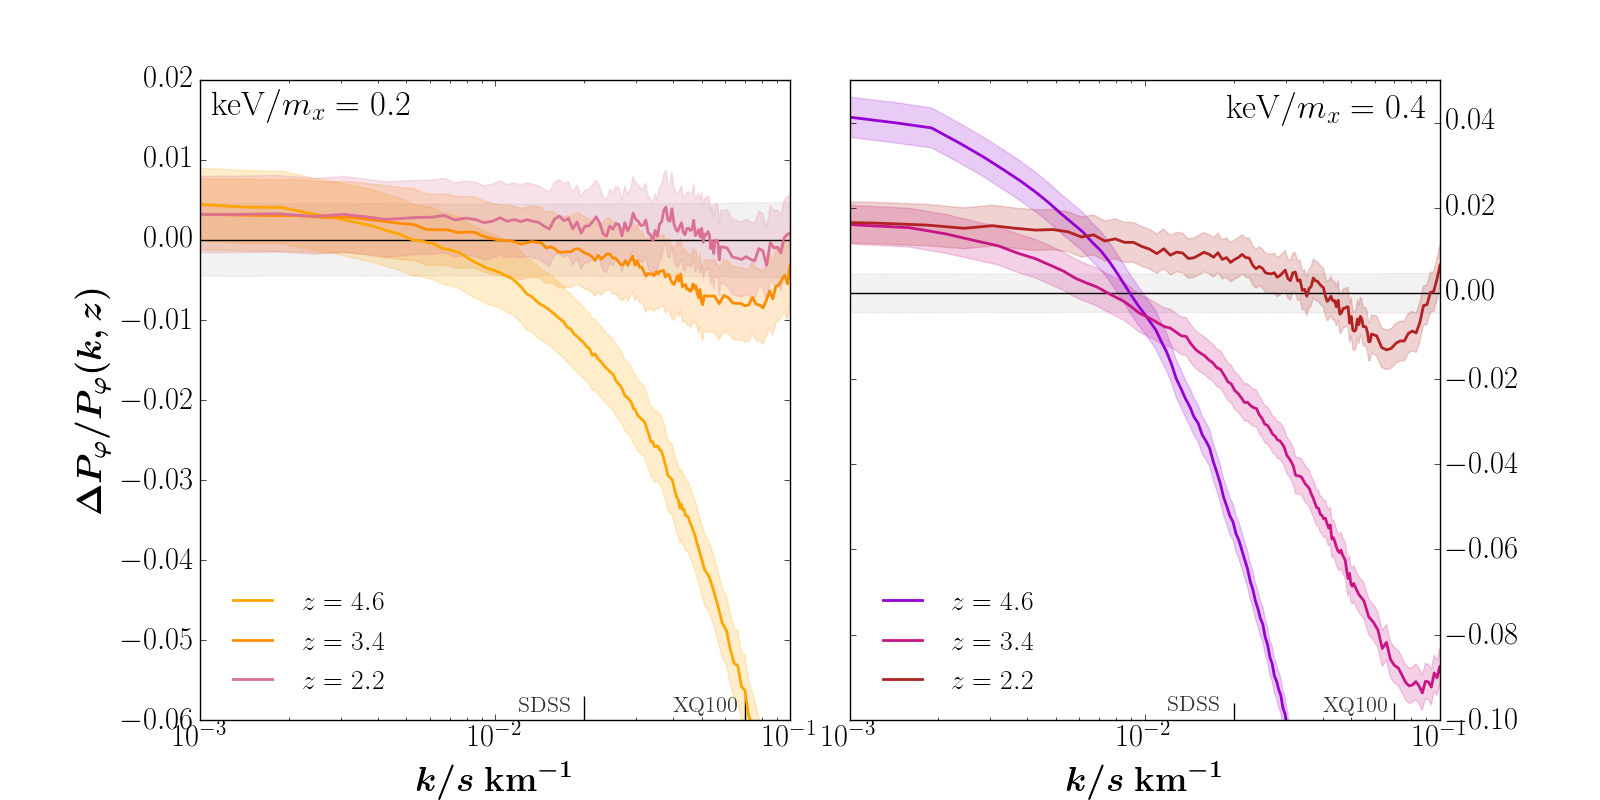
\includegraphics[width = 16cm]{WDM/Mx_Pf.png}
\caption{Relative difference in flux power spectrum with respect to the central \textit{best guess} model (black line) for $\mathrm{keV} / m_x = 0.2$ (left) and $0.4$ (right). Uncertainty on $P_\varphi (k)$ is encoded in the shade thickness. Color encodes redshifts $z=2.2, 3.4$ and $4.6$. The `SDSS' and `XQ100' ticks refer to the highest data $k$ mode in each survey.}
\label{fig:Mx_flux}
\end{center}
\end{figure}


\subsubsection{Limits with BOSS Data only}

Using our hydrodynamics simulations with $\mathrm{keV}/m_x > 0$ into our analysis, we obtain competitive lower limits on WDM mass. With Ly-$\alpha$+$H_0$ data (BOSS DR9), our $95\%$ C.L. are $m_x \geqslant 4.09~\mathrm{keV}$ for thermal relics and $m_{\nu_s} \geqslant 24.4 ~\mathrm{keV}$ for non-resonantly-produced sterile neutrinos, as shown in the first part of Tab.~\ref{tab:CL95_1D}. The fitted values of the nuisance parameters are all well within the expected range. The IGM nuisance parameters, the corrections to our model of the splicing technique and of the spectrograph resolution are all compatible with no correction at the $1\sigma$ level. The additive corrections to the estimate of the noise power spectra range from $-9\%$ to $+19\%$ with median at $-2.5\%$ and negligible correction in the redshift bins where the noise dominates over the signal (\textit{i.e.} at low redshift). The IGM temperature parameters have large error bars and are thus poorly constrained by this data set. Their values are within $1-2~\sigma$ of  typical  measurements (see \textit{e.g.} \cite{Becker2011}). Optical depth amplitude and index have consistent best-fitted values with those of our C+HDM case (see \ref{sec:mdm}) published in~\cite{Palanque2015b} (\textit{a.k.a.} $\Lambda$CDM$\nu$) although the uncertainty ranges are larger by a factor of 2 and 4 respectively: $A^\tau = \left( 25.0 \pm 2.6 \right) \times 10^{-4}$ and $\eta^\tau = 3.728 \pm 0.074$ ($68\%$ C.L.). \\

Our bounds on WDM mass were the most stringent at the time they were published in \cite{Baur16}. This was due in part to our large data sample and in part to our modeling of the flux power spectrum. \\
Modeling-wise, we benefited from an unprecedentedly large resolution for our SPH numerical simulations thanks in particular to or use of the splicing technique. Throughout my research, I've also contributed to greatly reducing several systematic effects which I've detailed in the previous chapter: the accuracy of the splicing method and the model of its residual by a scale-dependent  feature, the quantification of the sampling variance, the modelling of the IGM by a broken power-law, and a better accounting of the Hydrogen reionization history.  \\

\begin{table}[!]
\begin{center}
\begin{tabular}{lcccc}
\hline \\[-10pt]
\textbf{Data set} & \textbf{SDSS/BOSS} & \textbf{XQ-100} & \textbf{SDSS+XQ} & \textbf{SDSS+XQ+HR} \\[2pt]
\hline \\[-10pt]
$m_x / \mathrm{keV}$ & $4.09$ & $2.08$ & $4.17$ & $4.65$ \\[2pt]
$m^{\mathrm{nrp}}_{\nu_s} / \mathrm{keV}$ & $24.4$ & $10.2$ & $25.0$ & $28.8$ \\[2pt]
\hline \\[-10pt]
\end{tabular}
\end{center}
\caption{Lower bounds on a pure warm dark matter mass in units of keV, in the case of a thermal relic (first row) and a non-resonantly produced sterile neutrino (second row). All bounds are $95\%$ CL using the `Ly-$\alpha$ + $H_0$' data.}
\label{tab:Mx_limits}
\end{table}


Data sample wise, we benefited from a considerably larger Ly-$\alpha$ forest sample ($\sim 14,000$ in SDSS-III compared to $\sim 3,000$ in SDSS-I), two additional redshift bins ($z=4.2$ and $4.4$), and probing slightly lower scales; $k \leqslant 0.020 ~s/\mathrm{km}$ in SDSS-III compared to  $k \leqslant 0.018 s/\mathrm{km}$ in SDSS-I. We also carefully modeled the instrumental noise levels in each redshift bin and the uncertainty in the spectrograph resolution. As illustrated in Fig.~\ref{fig:Mx_flux}, the damping of small-scale perturbations due to free-streaming is more prominent at higher redshifts. As such, bounds on WDM particle mass are better constrained at higher redshifts, despite observations being more challenging. To quantify the beneficial impact of having two higher redshifts in our analysis, despite each one being very sparsely populated, we run our analysis by dropping both $\langle z \rangle = 4.2$ and $4.4$ bins and obtain the bounds listed in the second row of Tab.~\ref{tab:CL95_1D} labeled `$z \leq 4.1$': $m_x \geqslant 2.97~\mathrm{keV}$ and $m_{\nu_s} \geqslant 16.1~\mathrm{keV}$ ($95\%$ C.L.) which are $30\%$ less stringent than our bounds obtained with our full set labeled `$z \leq 4.5$'. \\

\begin{table}
\begin{center}
\begin{tabular}{lcc}
\hline \\[-10pt]
\textbf{Data set} & \multicolumn{2}{c}{ \textbf{Lower bound on $\; \cfrac{m_x}{\mathrm{keV}} \left( \cfrac{m^{\mathrm{nrp}}_{\nu_s}}{\mathrm{keV}} \right)$}}\\[2pt]
\hline \\[-10pt]
Ly-$\alpha$ + $H_0$ ($z \leq 4.5$) & \multicolumn{2}{c}{4.09 (24.4)} \\[2pt]
Ly-$\alpha$ + $H_0$ ($z \leq 4.1$) & \multicolumn{2}{c}{ 2.97 (16.1)} \\[2pt]
\hline \\[-10pt]
 & no running & with running\\[2pt]
Ly-$\alpha$ + $H_0$ + CMB {\scriptsize (TT + lowP)} & 2.96 (16.0) & 4.26 (25.7)\\[2pt]
Ly-$\alpha$ + $H_0$ + CMB {\scriptsize (TT + lowP+ TE + EE)} + BAO & 2.93 (15.8) & 4.12 (24.6)\\[2pt]
\hline \\[-10pt]
\end{tabular}
\end{center}
\caption{95\% C.L. lower bounds on thermal relic mass $m_x$, in keV, obtained with three data configurations. When Ly-$\alpha$ (BOSS DR9) is combined with other datasets, the limit is derived  with (right) or without (left) running of the spectral index. In each case, the corresponding NRP sterile neutrino mass (in keV) is given in parentheses (see Eq.~\ref{eq:mxms}).}
\label{tab:CL95_1D}
\end{table}


\subsubsection{Spectral Index Running}

\begin{figure}
\begin{center}
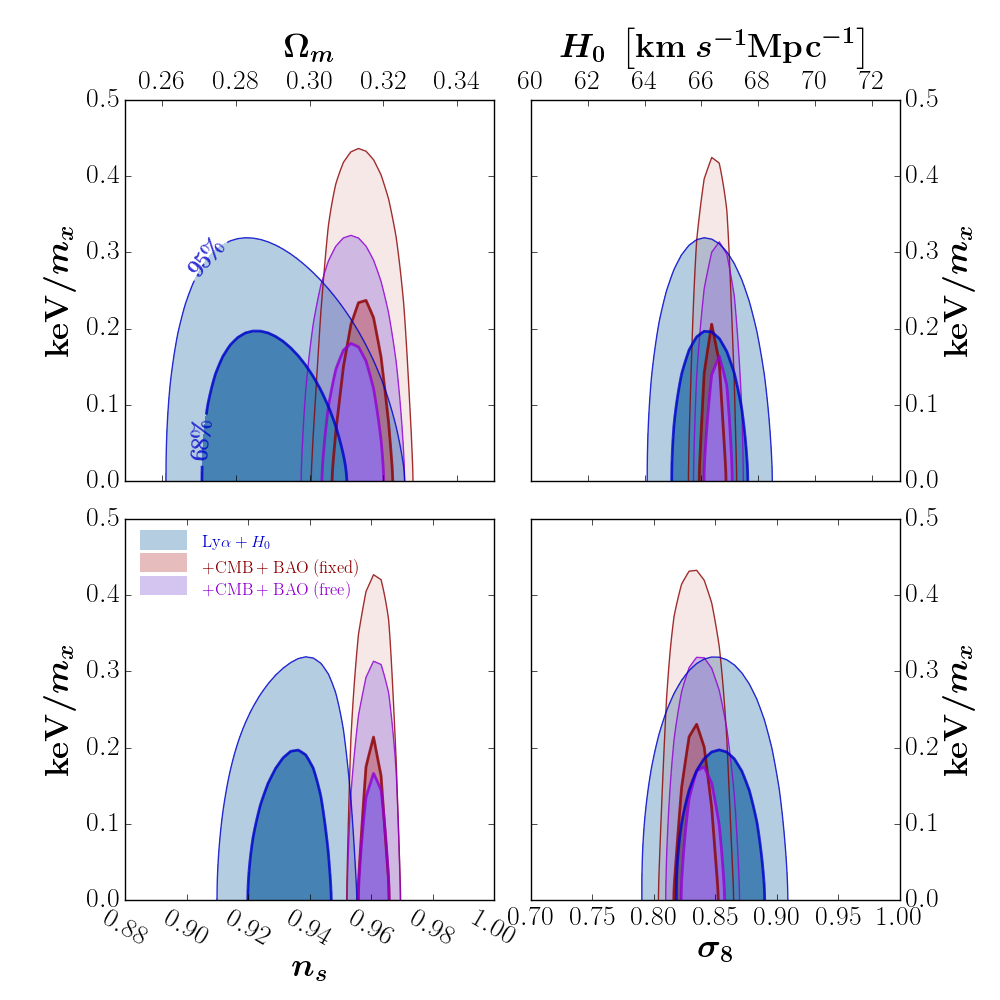
\includegraphics[width = 16cm]{WDM/C2D_All_zreio9.png}
\caption{$68\%$ and $95\%$ C.L. with regards to $1 \mathrm{keV} / m_x$ and the 4 cosmological parameters in our grid. Blue contours depict the Ly-$\alpha$ + $H_0$ bounds using BOSS DR9 data only. Red and purple contours are established by adding low-$\ell$ polarization, temperature and E auto and cross-correlation power spectra from Planck and measurements of the baryon acoustic oscillations scale, with the spectral index running $n_{\rm run}$ fixed to 0 (red) or allowed to vary (purple) and fitted as a free parameter in our multidimensional analysis.}
\label{fig:Contour_nrun}
\end{center}
\end{figure}

In addition to Ly-$\alpha$ forests, cosmic microwave background and baryon acoustic oscillations are other formidable probes to constrain cosmological parameters. These observations cannot directly probe the small scales at which WDM plays a role, and are therefore not expected to provide a direct constraint on the mass of a WDM particle. However, they can impact our constraint on WDM mass through the correlation of $m_{\mathrm{wdm}}$ with other cosmological parameters that are better constrained by CMB and BAO probes. We thus also include the Planck TT, lowP, TE and EE as well as measurements of the BAO scale (see Sec.~\ref{sec:data}). \\

Although these additional sets have contributed to establish competitive constraints on the sum of the masses of (standard) neutrinos $\sum m_\nu$ (see Sec.~\ref{sec:lcdmnu}) and the effective number of neutrino species $N_{\rm eff}$ \cite{Rossi2015}, they deteriorate our limit on WDM mass, which I've explicited in the last two rows of Tab.~\ref{tab:CL95_1D}, in the column labelled `no running'. This is the consequence of two factors: the tension on $n_s$ measured with Ly-$\alpha$ forest and the CMB on one hand, and the fact that our limit on the WDM mass is looser with increasing values of $n_s$ on the other hand (see the light tilt of the $2 \sigma$ contour in the lower left panel of Fig.~\ref{fig:Contour_nrun}). Combining CMB data increases the value of $n_s$ and thus loosens our limit on $m_x$. We measure no significant correlation between the value of running on the spectral index, which is set by the comparison of $n_s$ on large and small scales, and the value of $m_{\mathrm{wdm}}$ set by the shape and redshift-dependence of the power spectrum on scales probed by Ly-$\alpha$ data. \\

In the last two rows of Tab.~\ref{tab:CL95_1D}, I explicit the constraints on WDM mass obtained in the `no running' and `with running' configurations, which denote the cases in which the value of the spectral index running is either taken as fixed to zero or as a free parameter respectively. As expected, our limits on WDM mass when running is allowed to vary are similar to the limits that were derived from Ly-$\alpha$ data alone, since the effective value of $n_s$ on small scales is then determined by Ly-$\alpha$ data (and not by CMB data as in the `no running' case). We list in Tab.~\ref{tab:CL95_1D} the constraints obtained  for all three configurations (Ly-$\alpha$+$H_0$, Ly-$\alpha$+Planck with no running of $n_s$ and Ly-$\alpha$+Planck allowing for a running of $n_s$) to illustrate the impact of the value of $n_s$ on the sensitivity of our analysis. \\

Figure \ref{fig:Contour_nrun} displays the $68\%$ and $95\%$ C.L. bounds in the `with running' (purple) and `no running' (red) configurations in the $\left( \mathrm{keV}/m_x, \Omega_m \right)$, $\left( \mathrm{keV}/m_x, h \right)$, $\left( \mathrm{keV}/m_x, \sigma_8 \right)$ and $\left( \mathrm{keV}/m_x, n_s \right)$ planes. The contours for the Ly-$\alpha$+$H_0$ + CMB configuration are very similar to those for Ly-$\alpha$+$H_0$ + CMB + BAO (featured in the figure). The above discussion on the impact of spectral index running still holds true in the 2D case. More importantly, no significant correlation between our set of cosmological parameters and WDM mass is manifest, which conforts us in the interpretation that a small-scale power deficit in our simulated power spectrum would be due to the free-streaming of DM particles as opposed to a combined effect of $\Omega_m$, $H_0$, $\sigma_8$ and/or $n_s$. 


\subsubsection{IGM Thermal History}

\begin{figure}
\begin{center}
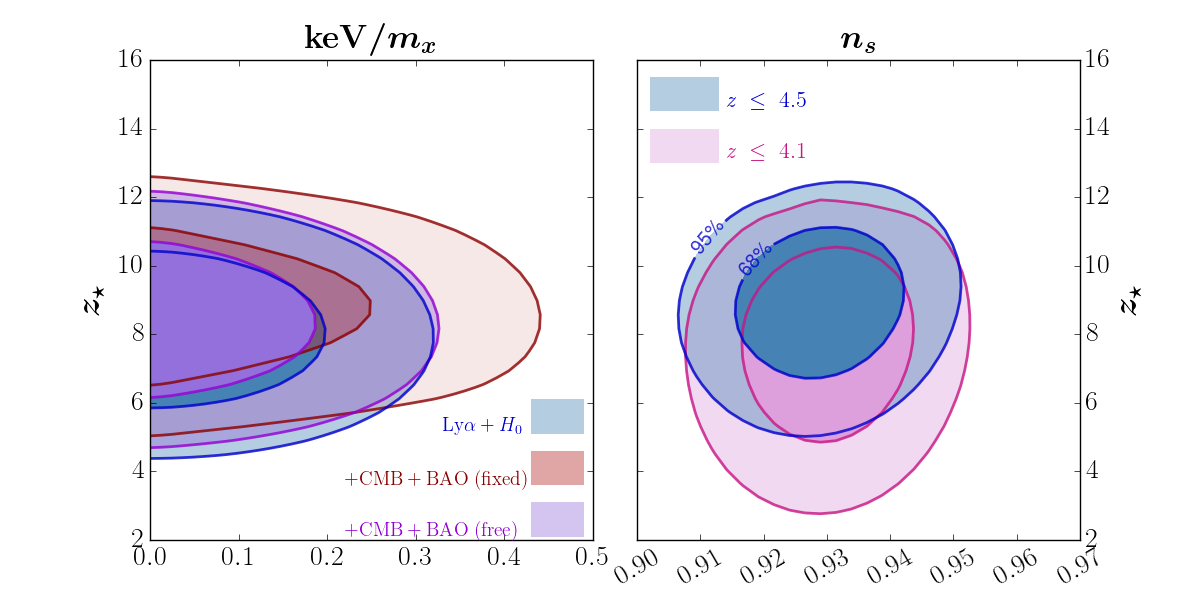
\includegraphics[width = 16cm]{WDM/C2D_Zreio9.png}
\caption{ Confidence intervals between the WDM mass (left) and the primordial spectral index (right) with the reionization redshift, given the same configurations as Fig.~\ref{fig:Contour_nrun}. The apparent lack of correlation is addressed in the text. The $z \leq 4.1$ (\textit{resp.} $4.5$) configuration corresponds to taking the first 10 (\textit{resp.} all 12) redshift bins from our data set (BOSS DR9 only).}
\label{fig:Contour_Zreio}
\end{center}
\end{figure}

One of the main challenge we face in establishing credible constraints on pure WDM particle mass is the uncertainty on the reionization history of the Universe. The redshift at which the ionizing UV background affects the Jeans smoothing scale of the baryon gas~\citep{Gnedin&Hui98} in a manner similar to the free streaming scale of warm dark matter particles. I've illustrated  this potential degeneracy in Fig.~\ref{fig:zreio_flux}. Fig.~13 of~\cite{McDonald2005} shows that an increase in the redshift of reionization from $z_{\star}=7$ to $17$ suppresses the Ly$\alpha$ flux power spectrum in the largest $k$-modes present in BOSS data ($k \sim 0.02~ s~\mathrm{km}^{-1}$) by about $1\%$ at $z=2.1$ and $4\%$ at $z=4.0$. In the present situation, however, the correlation between $z_\star$ and $m_x$ is strongly reduced for several reasons: \\

\begin{itemize}
\item[$\bullet$] our best-fitted value on $m_x$  ventures nearby the benchmark CDM model, showing no significant departure from $\mathrm{keV}/m_x=0$, which was explictely verified; \\

\item[$\bullet$] the data points with the highest statistical significance lie at low redshift where the correlation is the lowest; and \\

\item[$\bullet$] the many nuisance parameters that are fitted along with the cosmology and IGM parameters also contribute to absorbing the correlation.\\
\end{itemize}

More generally, these nuisance parameters render $z_\star$ to have relatively small correlations with all cosmological and astrophysical parameters. The strongest residual correlation is with the primordial spectral index $n_s$, at the $\sim 20\%$ level, which is expected since the effect of alternate values of $n_s$ on the flux power spectrum is a shift in the slope with respect to spatial scales. This slight correlation is manifest in the right panel of Fig.~\ref{fig:Contour_Zreio}, where the semi-major axis of the quasi-elliptical Ly-$\alpha$ contours deviates slightly from vertical. The correlation is damped when taking CMB data into account as it probes a $k$ range distinct from Ly-$\alpha$ forest data. \\


Our best-fit value for the redshift of reionization is $z_{\star} \simeq 8.2$ using BOSS data only. The best-fit value shifts to $z_{\star} \simeq 8.8$ and  $8.4$ in the fixed and fitted $n_{\rm{run}}$ Ly-$\alpha$+$H_0$+CMB configuration respectively, and to $z_{\star} \simeq 8.8$ and $ 8.5$ when BAO is also included, all consistent to within one standard deviation from the CMB constraint. As discused above, we detect no strong correlation between $z_{\star}$ and $m_x$, as shown on the left panel of Fig.~\ref{fig:Contour_Zreio}. We can quantify this statement using its global correlation coefficient, defined as the correlation between $z_\star$ and the linear combination of all other parameters which is most strongly correlated with it. We find that the global correlation coefficient for $z_\star$ is $60\%$. This  correlation is due to the fact that several other nuisance parameters in our fit encompass --- even partially --- the effect of the IGM thermal history on the transmitted flux power spectrum, namely the splicing residual pivot offset $r_{\epsilon} (k=k_p, z)$ and slope $dr_{\epsilon}/dk (z)$ (see Eq.~\ref{eq:splicing_dof}), as well as the uncertainties due to the redshift-dependence of the spectrograph resolution $\alpha_{\rm{reso}}$ and $\beta_{\rm{reso}}$. \\




\subsubsection{Warm Dark Matter or Warmer IGM ?}

\begin{figure}
\begin{center}
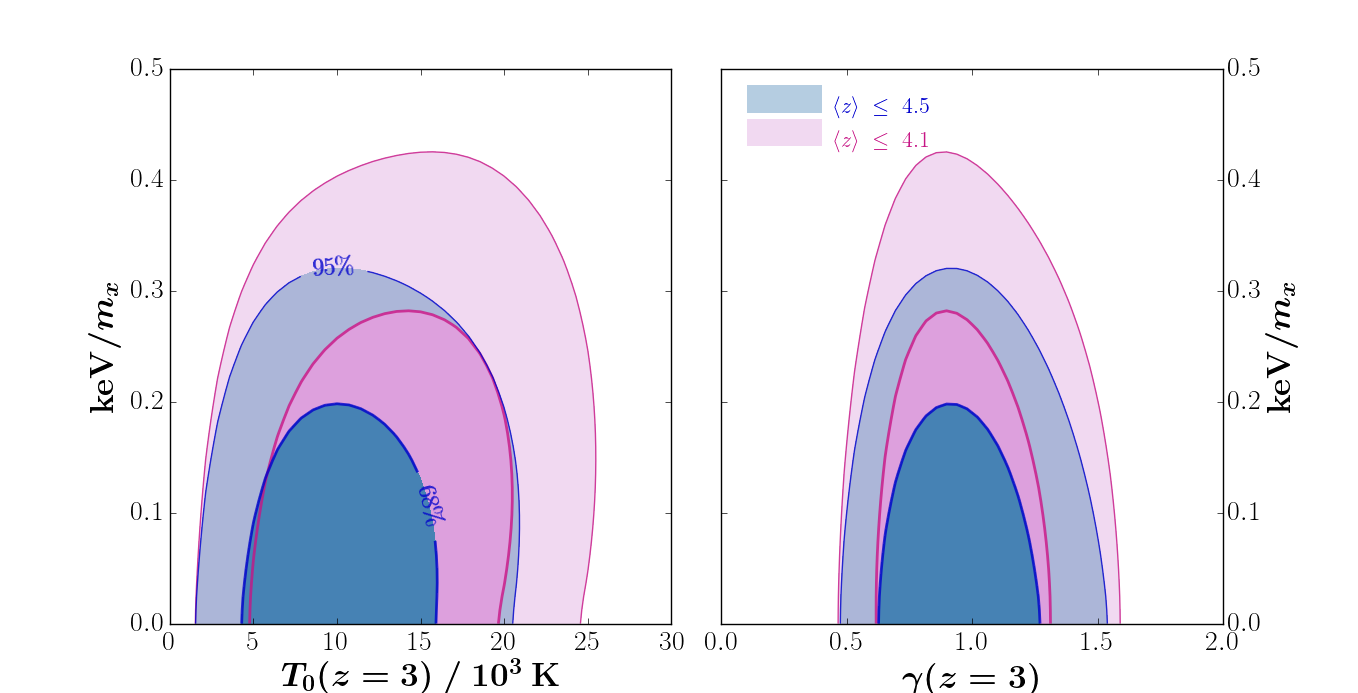
\includegraphics[width = 16cm]{WDM/C2D_IGM_zreio9.png}
\caption{ $68\%$ and $95\%$ C.L. bounds using the Ly-$\alpha$ + $H_0$ (BOSS only) configuration on $\mathrm{keV}/m_x$ with degeneracy on the two parameters modeling the evolution of IGM temperature with density input in our simulationss: mean background temperature $T_0^{z=3}$ (left) and index (right) $\gamma^{z=3}$. Blue (\textit{resp.} pink) contours correspond to the likelihood taking all 12 redshift bins (labelled `$z \leq 4.5$'), in comparison with excluding $\langle z \rangle = 4.2$ and $4.4$ (labelled `$z \leq 4.1$').}
\label{fig:Contour_T0gamma}
\end{center}
\end{figure}

It has been recently argued in \cite{warmIGM} that the small-scale cutoff in the power spectrum can be accounted for by a warm IGM rather than a warm DM particle. The temperature-density power-law defined in Eq.~\ref{eq:IGM} is a crude first-order assumption as the power-law intercept $T_0 \: (z)$ and exponent $\gamma \: (z)$ are poorly constrained. $T_0$ may not be a monotonic function of redshift at $z \gtrsim 5$. An extended apprehension of the thermal state of the IGM and its history is crucial in carrying out investigation in the lower velocity-space $k$ segments of the Ly-$\alpha$ flux power spectrum. In our likelihood computation, we allow the IGM temperature-density relation to obey two distinct power laws, above and below a $z=3$ break.
No degeneracy between IGM temperature at $z=3$ and WDM mass is manifest, as is illustrated in Fig.~\ref{fig:Contour_T0gamma}. Implementing the $\langle z \rangle = 4.2$ and $4.4$ bins into our multidimensional analysis tightens our bounds on WDM mass and lowers $T_0 \: (z=3)$ from $\sim 14,000$ to $\sim 10,000$ Kelvins. The temperature-density index $\gamma \: (z=3)$ remains unaltered. On all accounts, the issues raised in \cite{warmIGM} do not apply to the redshift and velocity-space ranges that we probe with BOSS alone. Our model of the IGM thermal state, although generic, is not the predominant limiting factor in the establishment of our bounds on WDM mass, as is apparent in Fig.~\ref{fig:Contour_T0gamma}. Our result is primarily limited by the sheer size and low resolution of our Ly-$\alpha$ power spectrum data sample.

\subsubsection{Adding the Higher Resolution Power Spectrum}

To better probe the cutoff scale caused by the particle free-streaming,
%To remedy the degeneracy of the impact of $m_x > 0$ on the flux power spectrum with the IGM temperature and reionization redshift, 
we make use of the higher resolution data sets introduced in Sec.~\ref{sec:data}.  For the  XQ-100 data set, where the power spectrum is measured down to $k \sim 0.07~s~\mathrm{km}^{-1}$ at $z=4.0$, we are very sensitive to the effect of $z_\star$. Adopting a method similar to the study of reionization by~\cite{McDonald2005}, we model the effect of reionization over the power spectrum using our $5$ hydrodynamics simulations with $z_{\star} = 8, 9, 12, 15$ and $16$. We introduce a nuisance parameter representing $z_{\star}$ which is let free in the likelihood computation with a constraint of $z_{\star} = 9.0 \pm 1.5$.  The central value and range of this external constraint are defined in order to encompass the most recent measurements of the redshift of reionization~\cite{WMAP9, Planck2015, Planck2016PolarReio}. \\


Using only the XQ-100 Ly-$\alpha$ forest power spectrum, along with $H_0 = 67.3 \pm 1.0 ~\mathrm{km}~s^{-1}\mathrm{Mpc}^{-1}$, yields a $95\%$ C.L. lower bound of $m_x \geqslant 2.08 ~\mathrm{keV}$ on thermal relics and $m_{\nu_s} \geqslant 10.2 ~\mathrm{keV}$ on NRP sterile neutrinos. These bounds are roughly twice looser than the bounds obtained using BOSS DR9 alone. However, combining both XQ-100 and BOSS DR9 Ly$\alpha$ forest power spectra, the $95\%$ C.L. limit is slightly improved compared to the one from BOSS DR9 alone: $m_x \geqslant 4.17~\mathrm{keV}$. The $99\%$ C.L. bounds are significantly improved, increasing from $m_x \geqslant 2.74 ~\mathrm{keV}$ for BOSS DR9 alone to $m_x \geqslant 3.10 ~\mathrm{keV}$ for the combined BOSS+XQ-100 data set.  The reason of this improvement is illustrated in the right panel of Fig.~\ref{fig:scan1dmx}, which shows the $\chi^2$ profile function of $\mathrm{keV}/m_x$ for the two data set configurations (BOSS alone and BOSS+XQ-100). Adding XQ-100 visibly increases its steepness but shifts the minimum's position into the physical ($\mathrm{keV}/m_x > 0$) region. This accounts for the small improvement of the $95\%$ C.L bound and the considerable improvement at higher significance ($3\sigma$ or more). Fitting the $\chi^2$ profile by $\Delta \chi^2 (\mathrm{keV}/m_X) =\chi^2_{\mathrm{min}} + (\mathrm{keV}/m_x-\mathrm{keV}/m_{x, \mathrm{min}})^2/\sigma^2+\alpha\cdot(\mathrm{keV}/m_x-\mathrm{keV}/m_{x, \mathrm{min}})^4$, the $\sigma$ parameter provides an estimator of the statistical sensitivity on $\mathrm{keV}/m_X$. The addition of XQ-100 allows us to reduce $\sigma$ from $0.15$ to $0.12$, representing a  $25\%$ gain in statistical sensitivity. \\

\begin{figure}
\begin{center}
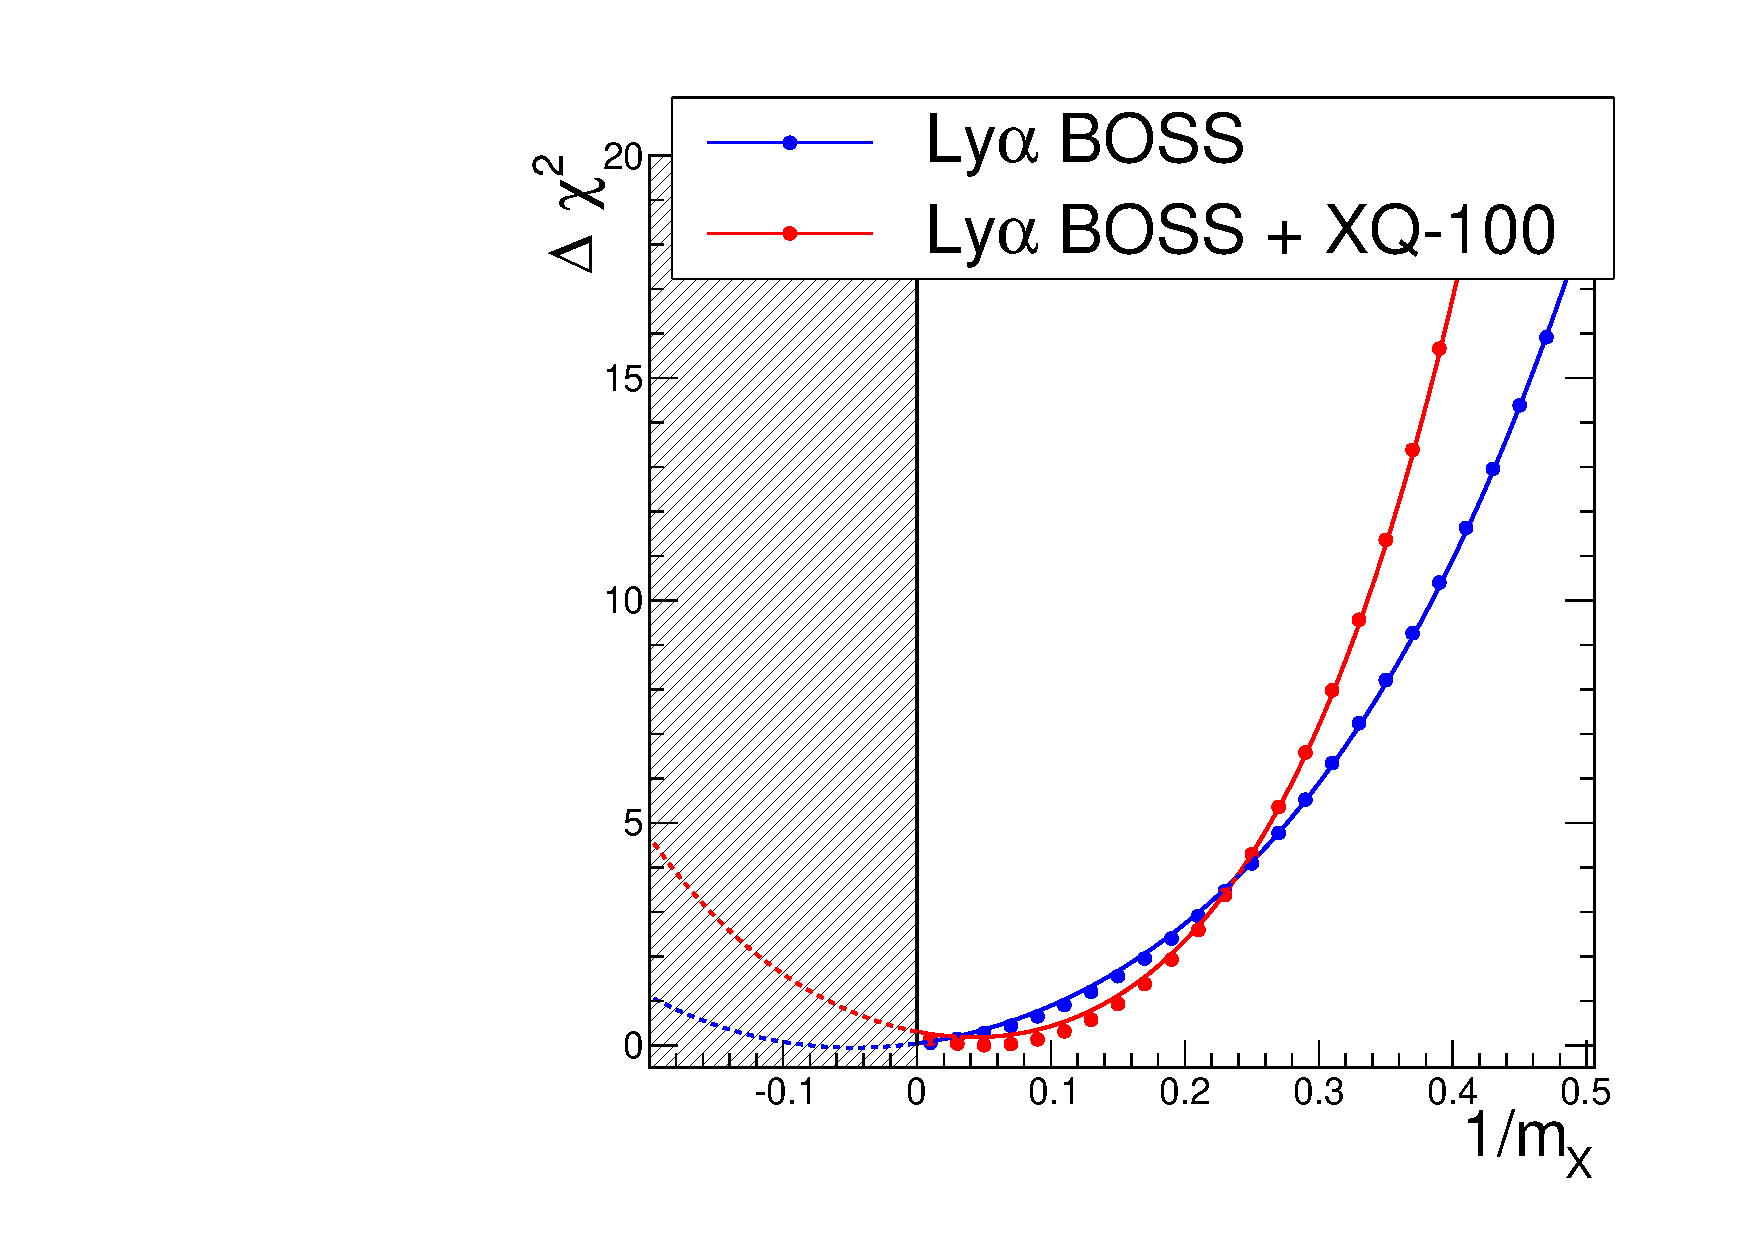
\includegraphics[width=0.85\columnwidth]{Mnu/Scan_1D_Chi2_invmx.pdf}
\caption{$\chi^2$ profile with respect to $\mathrm{keV}/m_x$}
\label{fig:scan1dmx}
\end{center}
\end{figure}


Although we believe that a Gaussian constraint with a sigma of 1.5 on $z_{\star}$ allows us to encompass the range of allowed $z_{\star}$ from CMB results (in particular~\cite{WMAP9, Planck2015, Planck2016PolarReio}), we  released the constraint on $z_{\star}$, allowing for a wider variation range, to study the impact on the warm dark matter mass bound. The effect is small: increasing $\sigma$ to $2.5$, the $95\%$ C.L. limit on $m_x$ decreases from $4.17 ~\mathrm{keV}$ to  $3.90 ~\mathrm{keV}$. \\

Finally, adding XQ-100 to BOSS data, we do not observe any significant change  in either the IGM temperature $T_0(z=3)$ or its index $\gamma(z=3)$ as a function of matter density. To investigate the hypothesis of a warmer IGM suggested in \cite{warmIGM}, additional Ly$\alpha$ forest data at higher redshifts ($z\ge 4.5$) is needed to better study  this hypothesis. \\

The analysis presented in~\cite{IrsicWDM} shows that the combination of the XQ-100 and HIRES/MIKE datasets can significantly improve the limit on $m_x$.  Indeed, the two datasets have different degeneracies between astrophysical and cosmological parameters that are disentangled when both data sets are combined, thanks to the higher resolution of the HIRES and MIKE spectrographs. In principle, adding the HIRES/MIKE Ly-$\alpha$ power spectrum to the combined BOSS DR9 + XQ-100 should improve our bounds. As was mentioned in Sec.~\ref{sec:data}, we can only make use of the two lowest redshift bins of the HIRES/MIKE data set ($z=4.2$ and $4.6$) since our hydrodynamics simulations do not go beyond the $z=4.6$ snapshot from \textsf{Gadget}. The Ly-$\alpha$+$H_0$ bounds we obtain using SDSS+XQ+HIRES/MIKE are $m_x \geqslant 4.65 ~\mathrm{keV}$ and $m_{\nu_s} \geqslant 28.8 ~\mathrm{keV}$ ($95\%$ C.L.).  The fit of the $\chi^2$ profile by a quadratic regression demonstrates a reduction of $\sigma$ from $0.123$ to $0.105$ and finally to $0.093$ when we add successively the $z=4.2$ and $z=4.6$ redshift bins of the high-resolution HIRES/MIKE data, representing a gain of respectively $17\%$ and $13\%$ in statistical sensitivity. In total, the statistical sensitivity gain with respecto to BOSS alone is $60\%$. The reason this substancial gain isn't reflected in our $95\%$ C.L. bound is once again due to the minimum $\chi^2$ position shifting from the $\mathrm{keV}/m_x < 0$ (unphysical) region to the $\mathrm{keV}/m_x > 0$ physical region. Our limit on $m_x$ is in agreement with the recently published bound $m_x \geqslant 5.3 ~\mathrm{keV}$  established in~\cite{IrsicWDM}. The main bottleneck issue WDM studies investigated by Ly-$\alpha$ forests face is incorporating the upper-most redshift bins from the high-resolution surveys and account for both the degeneracy of the WDM particle's free-streaming scale with both the Jeans length scale affected by the reionization redshift and the warmth of the IGM. This represents a substancial effort in both the observational front as well as the computational front, and specifically the modeling of the IGM's thermal history. Such improvements are beyond the scope of my PhD work, although I hope to have the opportunity to further investigate this area of research in the future. \\ 




%%%%%%%%%%%%%%%%%%%%%%%%%%%%%
\subsection{Cool Dark Matter}
\label{sec:res_rpsn}
%%%%%%%%%%%%%%%%%%%%%%%%%%%%%

The results on the pure WDM project I issued in the previous section assumes a generic warm dark matter particle. I've differentiated between an early-decoupled thermal relic, whose phase-space distribution function is a Fermi distribution; and a sterile neutrino produced in the early Universe by oscillations with the active neutrino masses. In Sec.~\ref{sec:rpsn_intro}, I've introduced the case of sterile neutrino production being boosted by a non-zero net lepton asymmetry in the early Universe. Resonantly produced sterile neutrinos (RPSN) as dark matter candidates are of particular interest these days since there is tentative evidence of the decay of a $7.1 ~\mathrm{keV}$ dark matter particle into $3.55~\mathrm{keV}$ neutrinos from the stacked X-ray spectra of galaxy clusters \citep{Bulbul14, Boyarsky14}. The X-ray flux (or lack thereof) also constrains the mixing angle of the sterile neutrino mass eigenstate and the other sub-$eV$ mass eigenstates, $\sin^2 2 \theta$. From the bounds on $m_{\nu_s}$ established in the previous section, if sterile neutrinos are the sole component of dark matter, then the un-boosted oscillation mechanism cannot account for the observed dark matter density, as manifest on the top black line in Fig.~\ref{fig:RPSN_MT}. So far, the most viable and straightforward production mechanism that allows for the available mixing angles is the aforementined resonance production introduced by \cite{ShiFuller99}. Investigating RPSN as pure dark matter is thus evidently worthwhile. Futhermore, no Ly-$\alpha$ forest power spectrum involving RPSN as cool dark matter had been produced with the full non-linear SPH treatment as of yet. I incorporated the 8 RPSN models listed in Eq.~\ref{eq:RPSN_models_simu} in Sec.~\ref{sec:offgrid} into our hydrodynamics simulations. In the present section, I detail the results from our analysis using the BOSS and BOSS+XQ-100+MIKE/HIRES data sets, with all the previously discussed caveats applying.\\

\subsection{Mapping between C+WDM and RPSN as cool DM}
\label{sec:mapping_flux_RPSN_CWDM}

If one assumes $\sim \mathrm{keV}$ sterile neutrinos account for dark matter, then one can thus expect either one of these 4 following possibilities: \\
\begin{itemize}
\item[$\bullet$] the sterile neutrino constitutes the entirety of dark matter ($F_{\rm{wdm}} = 1$) and is produced in absence of a net leptonic asymmetry ($\mathcal{L} = 0$);\\

\item[$\bullet$] the sterile neutrino constitutes $0 \leq F_{\rm{wdm}} < 1$ of the total dark matter and is produced in absence of a net leptonic asymmetry ($\mathcal{L} = 0$);\\

\item[$\bullet$] the sterile neutrino constitutes the entirety of dark matter ($F_{\rm{wdm}} = 1$) and is produced in presence of a net leptonic asymmetry in the early Universe $\mathcal{L} > 0$;\\

\item[$\bullet$] the sterile neutrino constitutes $0 \leq F_{\rm{wdm}} < 1$  of the total dark matter and is produced in presence of a net leptonic asymmetry in the early Universe $\mathcal{L} > 0$.\\
\end{itemize}

In Sec.~\ref{sec:pureWDM}, I explored the first of these 4 listed scenarios. The conclusion is that, to be consistent with Ly-$\alpha$ forest data from SDSS-III, the pure WDM sterile neutrino has to be more massive than $24.4~\rm{keV}$ with $95\%$ likelihood\footnote{the lower bound is relaxed to $16.0~\rm{keV}$ when adding CMB data}. This lower bound is at 12$\sigma$ tension with the upper bound issued by X-ray data, set at $4~\rm{keV}$. Scenario 1 has thus been strongly disfavored. Search for keV sterile neutrino DM has shifted to scenarios 2 or 3, which I investigated in two seperate projects: RPSN as cool dark matter which I comment in this current section; and the C+WDM project which I defer discussion to Sec.~\ref{sec:cwdm_flux}. \\

\begin{figure}
\begin{center}
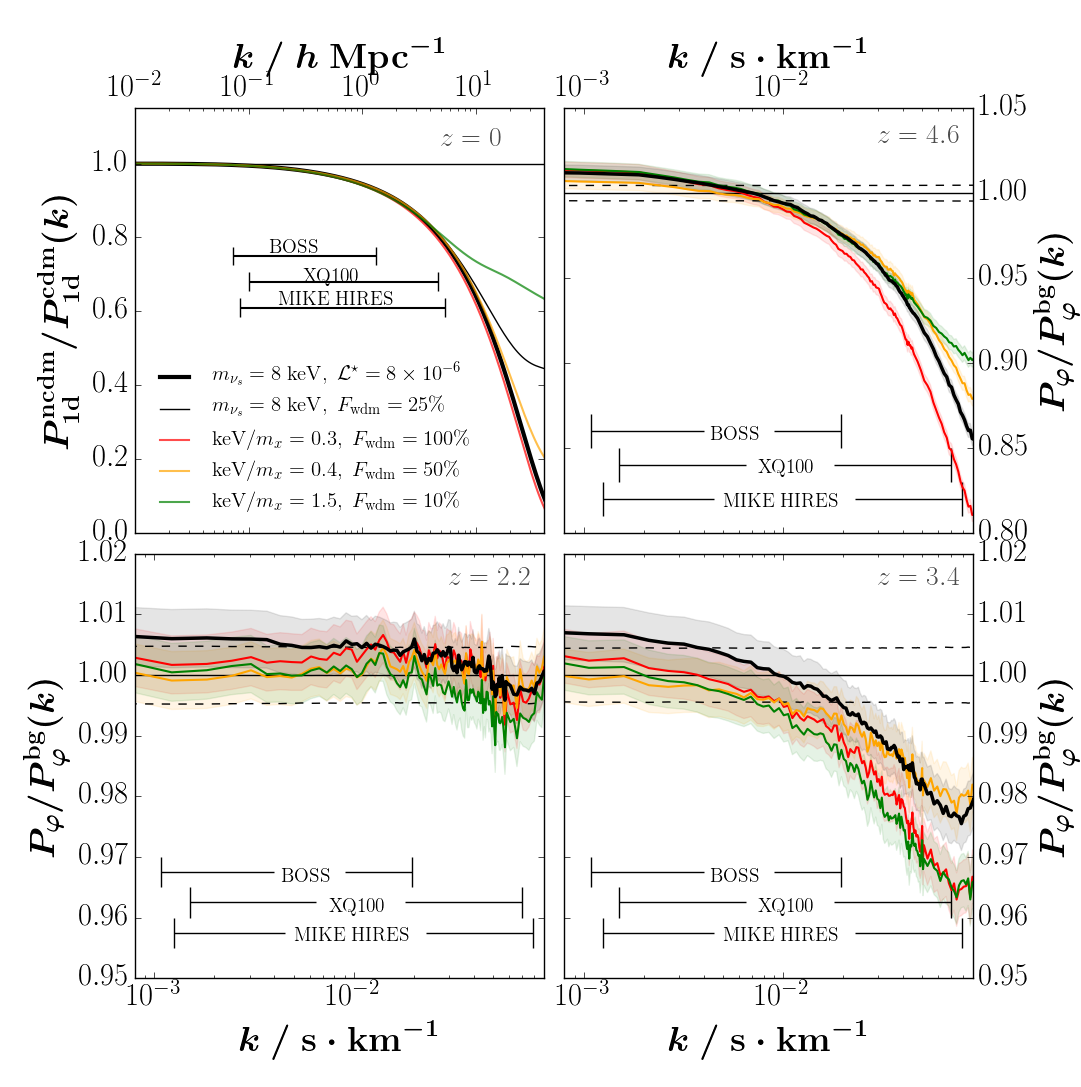
\includegraphics[width=\columnwidth]{RPSN/M8L8_quad.png}
\caption{Power spectra of the ($m_{\nu_s}/\mathrm{keV}=8$, $\mathcal{L}_6=8$) simulation normalized to the \textit{best guess} configuration, along with the ($\mathrm{keV}/m_x=0.3$, $F_{\rm{wdm}}=100\%$), ($\mathrm{keV}/m_x=0.4$, $F_{\rm{wdm}}=50\%$) and ($\mathrm{keV}/m_x=1.5$, $F_{\rm{wdm}}=10\%$) models. \textbf{Top Left:} 1D Linear matter power spectra ratio produced by \textsf{CLASS}. \textbf{Clockwise from Top Right:} Flux power spectra ratio produced by our hydrodynamical simulations at redshifts $z=4.6, 3.4$ and $2.2$. Shades encode simulation uncertainties (dotted lines for \textit{best guess}).}
\label{fig:flux}
\end{center}
\end{figure}


In Sec.~\ref{sec:map_rpsn_cwdm}, I described a mapping procedure between the free-streaming scale of RPSN and C+WDM models. This procedure involved the 1D linear transfer function of matter perturbations. This helped me guide my choice for the eight RPSN models chosen to run the SPH portion of the simulations, given that non-linear and baryonic effects were to be expected. Fig.~\ref{fig:flux} displays the resulting flux power spectrum (normalised by that of the \emph{best guess} simulation) for the M8L8$^{\star}$ simulation in black, along with several C+WDM models from Tab.~\ref{tab:cwdm_grid} featuring similar free-streaming scales. In the top left panel in Fig.~\ref{fig:flux}, the linear power spectra of the M8L8$^\star$ (in thick black) is shown along with the closest matching linear matter $T_{\mathrm{1d}}(k)$ of a C+WDM model assuming $m_{\nu_s} = 8~\rm{keV}$, which occurs for a warm-to-total DM fraction of $F_{\rm{wdm}} = 25\%$ (in thin black). As illustrated in Fig.~\ref{fig:M4t1d}, this linear transfer function correspondance is adequate up to some $k$ scale, beyond which the corresponding C+WDM model $T_{\mathrm{1d}}(k)$ breaks away from its comparative RPSN model to an asymptotical plateau ($T_{\mathrm{1d}}(k \rightarrow \infty) \propto (1-F_{\mathrm{wdm}}) \geqslant 0$). For most values of $m_{\nu_s}$ explored in this work, this breakaway $k$ is beyond the scales probed by our Ly-$\alpha$ forest data set, which I've materialized on the other three panels in Fig.~\ref{fig:flux}. I illustrate the negligible impact of differences in the linear 1D transfer function beyond the breakaway scale by overlaying three C+WDM models that exhibit similar $T_{\mathrm{1d}}$ on large scales but with significant (almost an order of magnitude) difference on the lowest scales.  The differences in the non-linear regime measured by the flux power spectra are within the statistical uncertainties of the simulations, almost an order of magnitude smaller than data uncertainties on similar scales. We thus expect no significant deviation, on the scales probd by our data sets, between the original RPSN hydrodynamics simulation (thick black) and its matching C+WDM one (thin black).\\


\begin{table*}
	\begin{center}
		\begin{tabular}{ccc}
			\textbf{RPSN model} & \textbf{SDSS} & \textbf{SDSS+XQ+HR}\\[2pt]
			\hline \\[-10pt]
			M4L12$^\star$ & $3.06 ~\sigma$ & $ >4\sigma$\\[2pt]
			M6L6 & $3.13 ~\sigma$ & $ >4\sigma$\\[2pt]
			M6L9$^\star$ & $2.0 ~\sigma$ & $3.3 ~\sigma$\\[2pt]
			M7L8$^\star$ & $1.9 ~\sigma$ & $3.1 ~\sigma$\\[2pt]
			M8L4 & $2.7 ~\sigma$ & $> 4 ~\sigma$\\[2pt]
			M8L8$^\star$ & $1.5 ~\sigma$ & $2.5 ~\sigma$\\[2pt]
			\hline \\[-10pt]
		\end{tabular}
	\end{center}
	\caption{Tension in standard deviations of the $P_{\varphi}(k)$ produced with 6 of our 8 hydrodynamics simulations in the RPSN configurations (column 1) with respect to the `SDSS only' (second column) and combined `SDSS+XQ+HR' (third column) data sets. I only show the configurations that fall between $1\sigma$ and $4\sigma$. }
	\label{tab:RPSNsigma}
\end{table*}


I use the interpolated $\chi^2$ levels in the $\left( \mathrm{keV}/m_x, F_{\mathrm{wdm}} \right)$ plane featured in Fig.~\ref{fig:chi2_WF} and transpose it into the $\left( m_{\nu_s}/\mathrm{keV}, \mathcal{L}_6 \right)$ plane using the mass mapping procedure described in Sec.~\ref{sec:map_rpsn_cwdm} and the $\chi2$ values obtained by the 8 RPSN models. The resulting likelihood 2D function is featured in Fig.~\ref{fig:RPSN_ML}. I compare the $\chi^2$ obtained 
using the RPSN power spectrum computed with our SPH simulations with that of its corresponding C+WDM model obtained with our mapping procedure in the linear regime, which Fig.~\ref{fig:flux} illustrates for the M8L8$^{\star}$ model. This cross-check between linear and non-linear mapping is done for both sets of data, SDSS/BOSS alone (`SDSS') and combined with VLT/XShooter, Keck/HIRES and LCO/MIKE (`SDSS+XQ+HR'). A systematic shift at the level of $0.2\,\sigma$ is observed in the first case, and of $0.5\,\sigma$ in the second, with the RPSN simulation showing a smaller $\chi^2$ (better agreement with the data) than its C+WDM matching counterpart. The better agreement for SDSS-only is consistent with a better match of the transfer function on large scales. The results I present in Fig.~\ref{fig:RPSN_ML} and hereafter for the RPSN models are corrected for this systematic shift. \\

\subsubsection{Constraints on Mass and Mixing Angle}


\begin{figure}
\begin{center}
  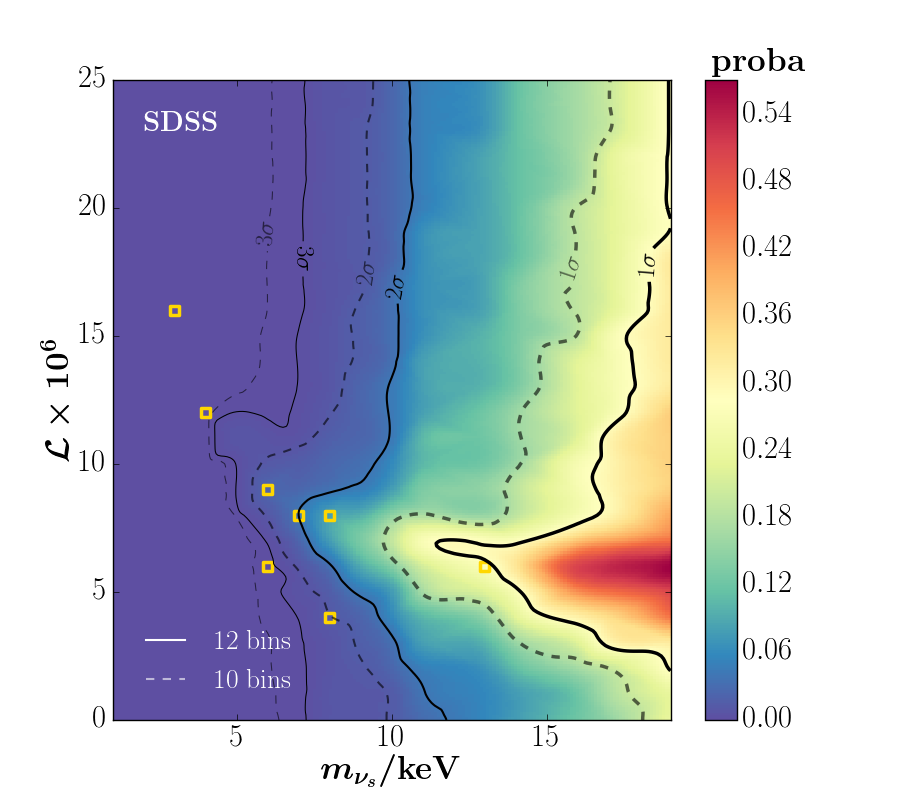
\includegraphics[width = 0.55\textwidth]{RPSN/Chi2_ML_boss.png}~%
  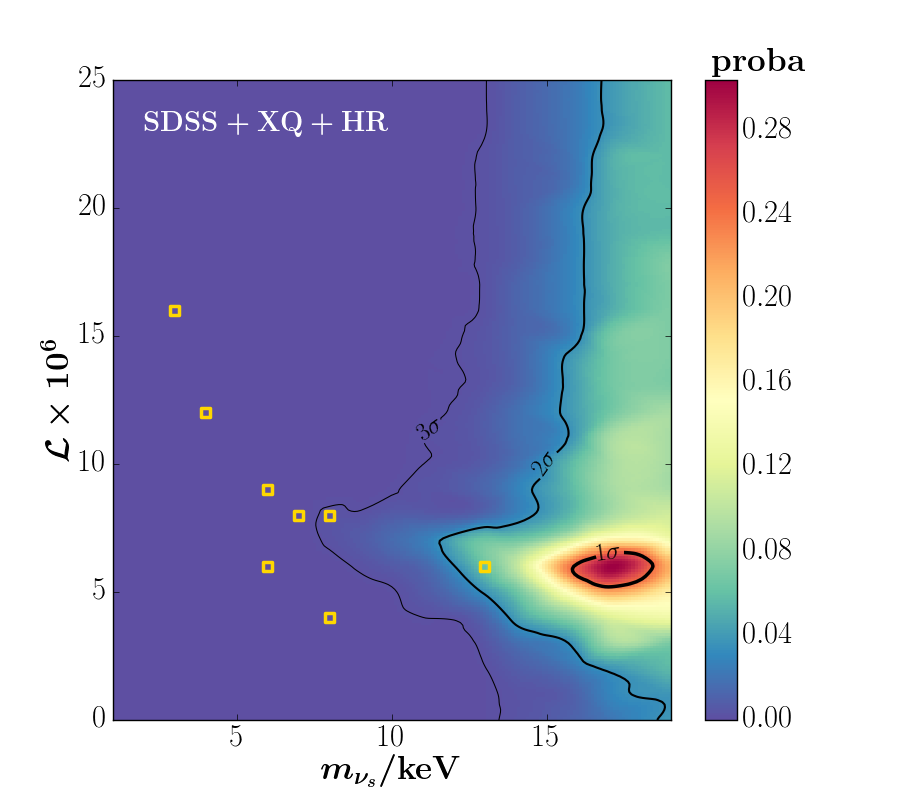
\includegraphics[width = 0.55\textwidth]{RPSN/Chi2_ML_bossxqhr.png}
  \caption{Constraints on ($m_{\nu_s}$, $\mathcal{L}$) obtained by the mapping
    described in Sec.~\ref{sec:mapping_flux_RPSN_CWDM}. Color encodes the values of the likelihood function described in Sec.~\ref{sec:methodology}. Gold squares map the 8 RPSN models we ran with our hydrodynamics simulations. \textbf{Left:} SDSS/BOSS data only. Solid curves are
    1, 2 and $3\sigma$ CL using all 12 redshift bins, while the dashed curves
    materialize the contours when excluding the 2 highest redshift bins ($z=4.2$
    and $4.4$) in the likelihood. \textbf{Right:} Combined SDSS (all 12 redshift bins) + XQ +
    HR data sets.
    }
\label{fig:RPSN_ML}
\end{center}
\end{figure}

Fig.~\ref{fig:RPSN_ML} displays the 1$\sigma$, 2$\sigma$ and 3$\sigma$ confidence level contours in the
($m_{\nu_s}$, $\mathcal{L}$) plane using our SDSS/BOSS Ly-$\alpha$
data  (left panel) or the full SDSS+XQ+HR  data (right
panel). The tension in standard deviations with these two data sets is reported in Table~\ref{tab:RPSNsigma} for the 4 relevant RPSN models for which I ran hydrodynamical simulations. A lepton asymmetry during the era of RPSN production in the early Universe
boosts the oscillation frequency from active to sterile neutrinos, thus
enabling ample production of dark matter sterile neutrinos with weaker mixing
angles $\theta$. Fig.~\ref{fig:RPSN_MT} displays the quantity $\sin^2 2 \theta$ as a function of $m_{\nu_s}$ assuming $\Omega_{\mathrm{dm}} h^2 = 0.26142 \times 0.675^2\simeq 0.119$ and values of the lepton asymmetry parameter in the range $0 \leq \mathcal{L} \leq 7 \times 10^{-4}$. The black lines in Fig.~\ref{fig:RPSN_MT} display the relation between  mass and mixing angle  for eight values of the primordial lepton asymmetry shown along each black curve (in  units of $10^{-6}$). The $\mathcal{L}_6 = 0$ thick line corresponds to non-resonant production. Values above $\mathcal{L} \gtrsim 10^{-3}$ are inconsistent with Big Bang nucleosynthesis (BBN). For $\sin^2 2 \theta \gtrsim 10^{-7}$, dark matter is overproduced. The region excluded by the Ly-$\alpha$ SDSS/BOSS data at the  $3\sigma$ CL is shaded in blue.  The dashed blue line indicates the limit using the 10 lowest redshift bins only, excluding $z=4.2$ and $4.4$. Values leftward of the red line are inconsistent with the Ly-$\alpha$ BOSS (12 bins) + XQ100 + MIKE/HIRES data at $\ge 3\sigma$ level, assuming the suppression observed in the high resolution data is  due to the thermal effects in the IGM (see discussion in~\cite{warmIGM}). \\


\begin{figure}[!]
\begin{center}
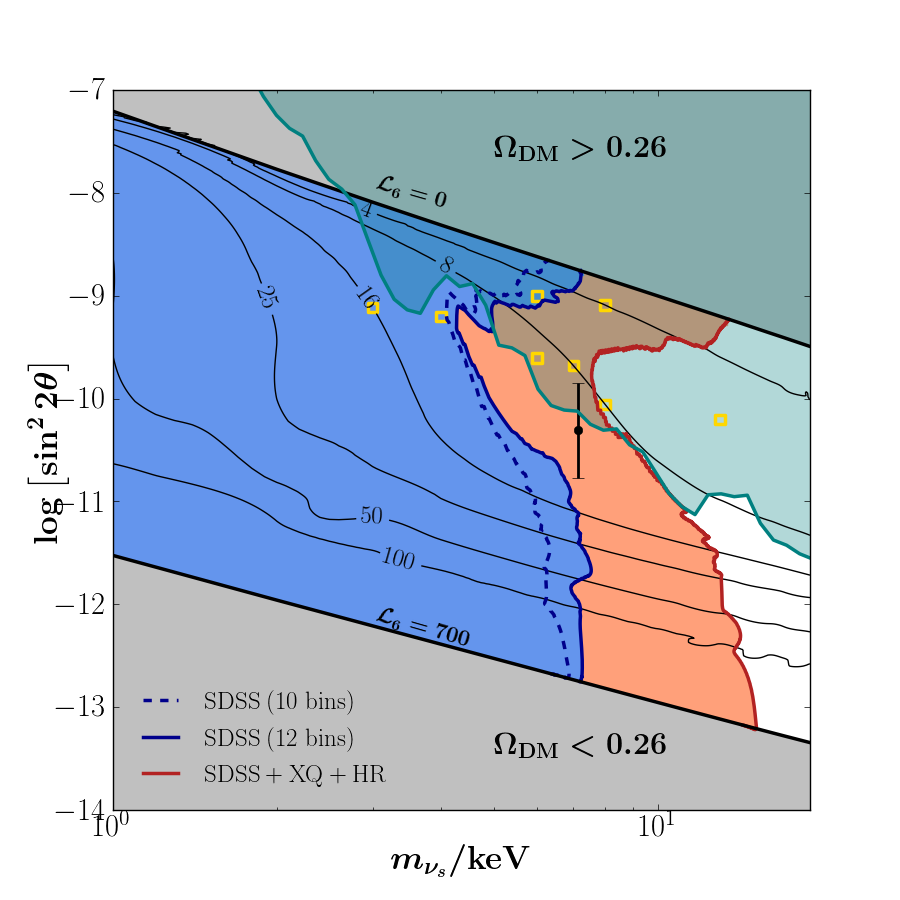
\includegraphics[width=\columnwidth]{RPSN/MS_3sigma.png}
\caption{Constraints from Ly-$\alpha$ forest in the RPSN ($m_{\nu_s}$,
  $\sin^2 2 \theta$) parameter space. The iso-$\mathcal{L}$ contours are displayed in black along with the corresponding value of $\mathcal{L}_6$. Gold squares indicate the set of parameters for which we computed the $P_\varphi (k)$ by solving the non-linear hydrodynamics. The black dot with error bar denotes the right-handed interpretation of the $3.55 ~\mathrm{keV}$ X-ray line in the stacked spectra of galaxy clusters, for which we used  $m_{\nu_s} = 7.14 \pm 0.07 ~\mathrm{keV}$ and $\sin^2 2 \theta = 4.9^{+ 1.3}_{-1.6} \times 10^{-11}$ as reported in \cite{Boyarsky14}. The blue (\textit{resp.} red) shade encompasses  models excluded by over $3\sigma$ by the SDSS-only (\textit{resp.} SDSS + XQ + HR) Ly-$\alpha$ forest  power spectrum. The absence of monochromatic X-ray lines (apart from the  $3.55~\mathrm{keV}$ signal) translate into upper bounds in $\sin^2 2 \theta (m_{\nu_s})$: the green shade are models inconsistent beyond $3\sigma$ with a compilation of X-ray data from the Milky Way, Andromeda and other galaxies.}
\label{fig:RPSN_MT}
\end{center}
\end{figure}



As expected from the white stripe visible on the right panel of Figs.~\ref{fig:rpsn_banana} and~\ref{fig:L_to_F_map}, the coolest RPSN models, which occur for $\mathcal{L} = \mathcal{L}^{\star}(m_{\nu_s})$, feature the longest free-streaming length and are more consistent with Ly-$\alpha$ forest data than other values of $\mathcal{L}$. This is manifest on Fig.~\ref{fig:RPSN_ML} (left panel) as a horn-like valley in the $\chi^2$ map, which extends to sterile neutrino masses around $\sim 7~\mathrm{keV}$ in the right-hand panel. This area  is of particular interest since it matches the range of masses and mixing angles for which the $3.55~\mathrm{keV}$ X-ray  signal reported in \cite{Bulbul14, Boyarsky14, Boyarsky2015}  can be interpreted as photons emitted by the decay of a $7.1~\mathrm{keV}$ right-handed neutrino. Although this region exhibits a $\sim3\sigma$ tension with the SDSS+XQ+HR Ly-$\alpha$ data, two  caveats should be considered. First,  IGM thermal histories impact the small scales ($0.02 ~\leq~ k / s~\mathrm{km}^{-1}~ \leq~ 0.07$) probed by these high-resolution data. Although we marginalize over 5 parameters to describe the thermal history  (as explained above), more general models (non-monotonic temperature evolution for instance) could loosen our constraint. Second, the flux power spectrum exhibits large gradients with respect to the RPSN parameters around the ``horn" region,  where the interpolation procedure is thus more delicate.
Therefore, because of the interest of this region for RPSN constraints, we located our eight RPSN simulations in that area: six correspond to the coolest models for their mass  (M3L16$^\star$, M4L12$^\star$, M6L9$^\star$, M7L8$^\star$, M8L8$^\star$ and M13L6$^\star$), the remaining two (M6L6 and M8L4) being slightly warmer than their corresponding counterparts at the same mass (M6L9$^\star$ and M8L8$^\star$). 
The results presented in Table~\ref{tab:RPSNsigma} show that the horn is a real feature,  although the exact location of its boundaries might require additional hydrodynamical simulations to assess. 
Hence the shape of the blue and red contours on Fig.~\ref{fig:RPSN_MT} may be less accurate  in the regions around the 6 bottom-most gold squares that correspond to our coolest RPSN models. 
The neutrino decay origin of the $3.55~\mathrm{keV}$ X-ray line, shown as the black dot with error bars, is located in this  region. \\

For the reasons just stated, I suggest scanning the  area  around  $m_{\nu_s} = 7.1  ~\mathrm{keV}$ and $\sin^2 2 \theta = 4.9 \times 10^{-11}$ with a set of dedicated hydrodynamical simulations in order to properly account for the strong dependence of the power spectrum on model parameters in that region. These simulations should also implement the different IGM thermal histories prognosticated in \cite{warmIGM}. I leave this outlined prognosis for future work.


%As expected from the white stripe visible on the right panel of Figs.~\ref{fig:rpsn_banana} and~\ref{fig:L_to_F_map}, the coolest RPSN models, which occur for $\mathcal{L} = \mathcal{L}^{\star}(m_{\nu_s})$, feature the longest free-streaming length and are more consistent with Ly-$\alpha$ forest data than other values of $\mathcal{L}$. This is manifest on Fig.~\ref{fig:RPSN_ML} (left panel) as a horn-like valley in the $\chi^2$ map from the SDSS/BOSS data.
%Using the combined data set issues a local maximum in the likelihood around $\sim 8~\mathrm{keV}$ visible as a small $3\sigma$  ``island'' in the right-hand panel of Fig.~\ref{fig:RPSN_ML}. This area  is of particular interest since it matches the range of masses and mixing angles for which the $3.55~\mathrm{keV}$ X-ray  signal reported in \cite{Bulbul14,Boyarsky14,Boyarsky2015}  can be interpreted as photons emitted by the decay of a $7.1~\mathrm{keV}$ right-handed neutrino. Although this region exhibits a $\sim3\sigma$ tension with the SDSS+XQ+HR Ly-$\alpha$ data, two major caveats should be considered. First,  IGM thermal histories impact the small scales ($0.02 ~\leq~ k / s~\mathrm{km}^{-1}~ \leq~ 0.07$) probed by these high-resolution data. Although we marginalize over 5 parameters to describe the thermal history, more general models (non-monotonic temperature evolution for instance) could loosen our constraint. Second, the flux power spectrum exhibits large gradients with respect to the RPSN parameters around the ``horn" region. Therefore the interpolation procedure might be more approximate in this region. Since the ``horn'' is nevertheless the region of interest for RPSN constraints, we located our eight RPSN simulations in that area: six correspond to the coolest models for their mass, the remaining two (M6L6 and M8L4) being slightly warmer than their corresponding counterparts (M6L9$^\star$ and M8L8$^\star$). This choice makes us confident that the horn on the left panel and the $3\sigma$ island on the right panel are real features (see Table~\ref{tab:RPSNsigma}). However, the interpolation method might fail to capture the drastic changes of free-streaming length when scanning values of mass and leptonic asymmetry around them.  Hence the shape of the blue and red contours on Fig.~\ref{fig:RPSN_MT} may be less accurate  in the regions around the 6 bottom-most gold squares, which correspond to our coolest RPSN models. The neutrino decay origin of the $3.55~\mathrm{keV}$ X-ray line, shown as the black dot with error bars, is located in this hazardous region. \\

%For the reasons just stated, I suggest scanning the hatched region in the $m_{\nu_s} - \sin^2 2 \theta$ parameter space with a set of dedicated hydrodynamical simulations in order to properly account for the strong dependence of the power spectrum on model parameters in that region. These simulations should also implement the different IGM thermal histories prognosticated in \cite{warmIGM}. I leave this outlined prognosis for future work.

\clearpage